\documentclass[onecolumn]{revtex4-2}
\usepackage{amsmath}
\usepackage{graphicx}
\renewcommand{\vec}[1]{\boldsymbol{#1}}
\begin{document}
\title{Summary of results}
%\author{Christopher K\"orber}
\maketitle

\section{Operator definitions}

All of the results are very preliminary and may be off by a factor.
I need to run further cross-checks.
For now, these plots should rather indicate the $q^2$ scaling.

\subsection{One-Nucleon operators}
Kinematics for single-nucleon system
\begin{equation}
    N(\vec p_1) + J(\vec q) \to N(\vec p_1')
\end{equation}

Operator definitions
\begin{align}
    \mathcal{O}_{1N}^{(1)}
    &=
    1
    \,\\
    \mathcal{O}_{1N}^{(DF)}
    &=
    \frac{k^2}{8 m_N^2}
    \,\\
    \mathcal{O}_{1N}^{(SO)}
    &=
    \frac{i}{4 m_N^2} \vec \sigma_1 \cdot (\vec q \times (\vec p_1 + \vec p_1'))
    =
    \frac{i}{2 m_N^2} \vec \sigma_1 \cdot (\vec q \times \vec p_1 )
\end{align}
where $\vec \sigma_1$ is the Pauli (spin) matrix of the first nucleon.

\subsection{Two-Nucleon operators}

Kinematics for two-nucleon system
\begin{equation}
    N(\vec p_1) + N(\vec p_1) + J(\vec q) \to N(\vec p_1') +N(\vec p_2')
\end{equation}

Operator definitions
\begin{align}
    \mathcal{O}_{2N}^{(1\pi_1)}
    &=
    \frac{-3 g_A^2}{16 F_\pi^2 m_N}
    \frac{(\vec \sigma_1 \cdot \vec q)(\vec \sigma_1 \cdot \vec q_2)}{\vec q_2^2 + M_\pi^2}
    + (1 \leftrightarrow 2)
    \,\\
    \mathcal{O}_{2N}^{(1\pi_2)}
    &=
    \frac{-3 g_A^2}{16 F_\pi^2 m_N}
    \frac{(\vec \sigma_1 \cdot \vec q_2)(\vec \sigma_2 \cdot \vec q_2)(\vec q_2 \cdot \vec k)}{\vec q_2^2 + M_\pi^2}
    + (1 \leftrightarrow 2)
\end{align}
with $\vec q_1 = \vec p_1' - \vec p_1$ and $\vec q_2 = \vec p_2' - \vec p_2$ and
\begin{align}
    \mathcal{O}_{2N}^{(A)}
    &=
    2 \vec q^2 \to 2 F_1(\vec p_{12}, \vec p_{12}', \vec q)
    \, , \\
    \mathcal{O}_{2N}^{(B)}
    &=
    2 \vec q^2 (\vec \sigma_1 \cdot \vec \sigma_2) \to 2 (\vec \sigma_1 \cdot \vec \sigma_2) F_1(\vec p_{12}, \vec p_{12}', \vec q, \Lambda)
    \, , \\
    \mathcal{O}_{2N}^{(C)}
    &=
    2 (\vec \sigma_1 \cdot \vec q)(\vec \sigma_2 \cdot \vec q) \to 2 F_2(\vec p_{12}, \vec p_{12}', \vec q, \Lambda)
\end{align}
and $\vec p_{12} = (\vec p_1 - \vec p_2)/2$

\section{Parameters}
\begin{align}
    \hbar c &= 197.327 [\mathrm{MeV} \, \mathrm{fm}]\, , &
    m_N &= 938.918 \, [\mathrm{MeV}] \, , &
    g_A &= 1.29 \, , &
    m_\pi &= 138.03 \, [\mathrm{MeV}] \, , &
    F_\pi &= 92.4 \, [\mathrm{MeV}] \, .
\end{align}

\section{Wave function}

Example wave function string:

\texttt{compton-dens-4he-chsms-n4lo+-cut=4-pCoul-n2locmpi-Lam=550.000}

\texttt{-c1=-1.230-c3=-4.650-c4=3.280-Lamnum=1.000e+08-tnfcut=3}

\texttt{-om=1.60E+00-th=1.80E+02-nx=20-nphi=16-np12=np34=28+8-np3=44+8-nq4=nq=38+6-}

\texttt{j12max=5-lmax=6-lsummax=12-tau4max=0-rho1b.dat}

\begin{table}[htb!]
    \caption{The following matrix elements will be evaluated for the wave function}
    \label{}
    \begin{tabular}{ll}
    nuc       &       4he \\
    potential &     chsms \\
    order     &     n4lo+ \\
    empot     &     pCoul \\
    cmpi      &  n2locmpi \\
    tnfcut    &         $3$ \\
    cut       &        $4$\\
    \end{tabular}$\quad$
    \begin{tabular}{ll}
    $n_{p_{12}} = n_{p_{34}}$ &      $28+8$ \\
    $n_{p_{3}}$       &      $44+8$ \\
    $n_{q_4} = n_q$   &      $38+6$ \\
    $\Lambda$       &       $550$\\
    $c_1$        &  $-1.23$ \\
    $c_3$        &  $-4.65$ \\
    $c_4$        &  $3.28$
    \end{tabular}
\end{table}

\section{Results}

\subsection{One-nucleon leading contributions}

For the leading 1N contribution $\mathcal{O}_{1N}^{(1)}$ I have performed a polynomial fit to see with which precision one can extract the form factor and radius.

According to a previous mail, I have rescaled the FF to be one at the origin (original norm: $F(0) = 0.9988586308$).

To estimate the uncertainty of the fit parameters, I need to estimate the size of the numerical errors.
These errors are estimated employing an emperical Bayes scheme (e.g., optimize $\chi^2_{d.o.f} \to 1$ for best fits as a function of the unkown data error).
I make the assumption that all numerical errors are independent of $q^2$ and uncorrelated (which is likely not true but should suffice as a magnitude of order check).
For an even polynomial of order 4, I obtain that the \textit{data-error} $\Delta y \approx 5.6 \cdot 10^{-7}$.
Using this error, I have fitted several even polynomial of order 2 to 8 to the data.
They seem to stabilize around order 4 though there seems to be a significant difference (not captured by the parameter uncertainty) hoping from order 2 to 4.
The best value I can extract is
\begin{equation}
    r0 = \sqrt{-6 c_1}  = 1.42077(35) [\mathrm{fm}]\,.
\end{equation}
However, this estimate makes the assumption that the emperical Bayes method estimates the numerical uncertainty correctly.
Likely, the data uncertainty is larger and thus the parameter value uncertainty is larger as well.

\begin{figure}[htb!]
    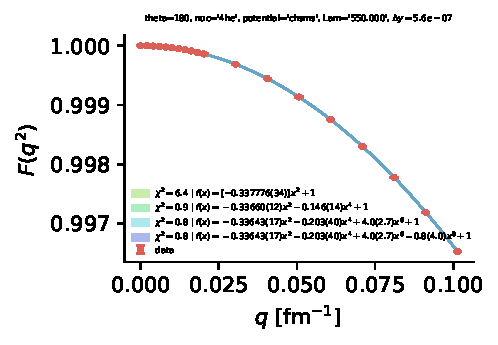
\includegraphics{figs/multi-poly-fit.pdf}
    \caption{Leading 1N contributions and FF fit.}
    \label{}
\end{figure}

\subsection{One-nucleon subleading contributions}
\begin{figure}[htb!]
    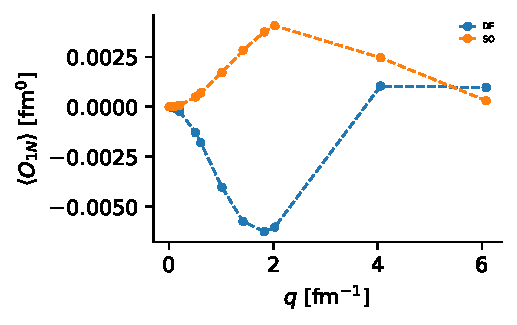
\includegraphics{figs/1n-nlo.pdf}
    \caption{Subleading 1N contributions.}
    \label{}
\end{figure}

\subsection{Two-nucleon one-pion exchange}
\begin{figure}[htb!]
    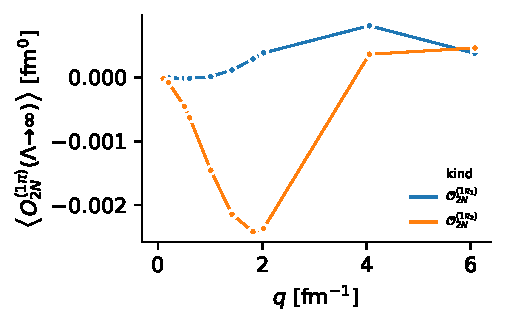
\includegraphics{figs/2n-ope.pdf}
    \caption{2N OPE contributions for infinite cutoff.}
    \label{}
\end{figure}

\subsection{Two-nucleon contact}
\begin{figure}[htb!]
    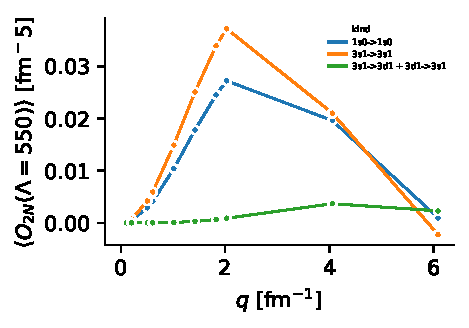
\includegraphics{figs/2n-contact.pdf}
    \caption{2N contact contributions for cutoff matching wave function.}
    \label{}
\end{figure}

\end{document}
